\documentclass{beamer}

% Russian-specific packages
\usepackage[T2A]{fontenc} % поддержка специальных русских символов
\usepackage[english,russian]{babel}
\usepackage[utf8]{inputenc}

% русские переносы
\usepackage{hyphenat}
% \hyphenation{ма-те-ма-ти-ка вос-ста-нав-ли-вать}

% Стиль презентации
\usetheme{Warsaw}
\usecolortheme{crane}

\begin{document}

% Оформление титульного листа
\title[Развитие ППРЭ]
{Развитие метода разностной эволюции
для поиска параметров математических моделей}
\author[Свичкарев Анатолий]
{Студент: \textbf{Свичкарев Анатолий, группа 53601/4}\\
Научный руководитель: \textbf{Козлов Константин Николаевич}}
\institute[СПбПУ]
{Санкт-Петербургский Государственный
Политехнический Университет\\Петра Великого}
\date{март, 2016}

% Создание заглавной страницы
\frame{\titlepage} 

\begin{frame}{Введение}
Математические модели в биоинформатике в
большинстве случаев создаются в таких компьютерных
системах расчетов как \textbf{R, MATLAB, Octave} и др.
\bigskip

Нахождение параметров в таких моделях требует
многократного вычисления решений, что влечет
большие накладные расходы на запуск того или иного
интерпретатора.
\end{frame}

\begin{frame}{Цель}
\textbf{Развитие метода ППРЭ}

\bigskip
За счет единовременной загрузки
неизменяемых данных и
асинхронной загрузки переменных параметров
планируется достигнуть
\textbf{сокращения времени вычисления}
при использовании
интерпретируемых языков, например,
для системы статистических расчетов R.
\end{frame}

\begin{frame}{Задачи}
\begin{enumerate}
    \itemsep 2em
    \item реализовать расширение программы ППРЭ,
        позволяющее запускать нужное количество копий
        интерпретатора один раз при старте.
    \item провести численные эксперименты с тестовыми функциями
    \item провести сравнительный анализ полученных результатов
\end{enumerate}
\end{frame}

\begin{frame}{Разностная эволюция}
    \begin{block}{Разностная эволюция}
        --- стохастический итерационный алгоритм минимизации,
        предложенный Сторном и Прайсом в 1995 г.
    \end{block}
    \begin{figure}[!h]
        \centering
        % TODO максимальный доступный размер
        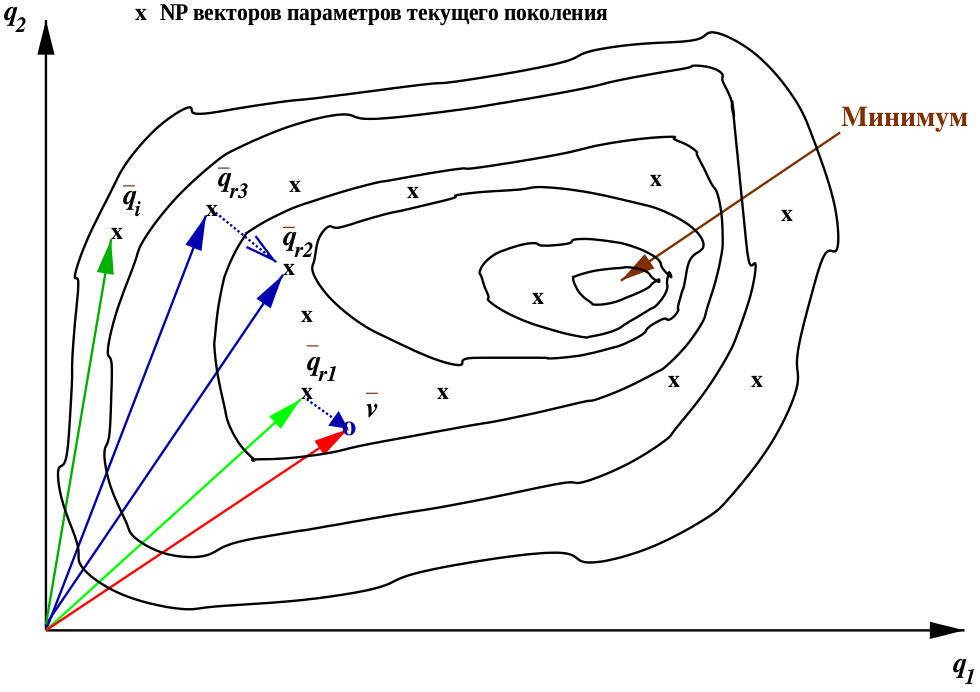
\includegraphics[scale=0.2]{DE}
        \caption{Геометрическая интерпретация метода разностной эволюции}
    \end{figure}
\end{frame}

\begin{frame}{Полностью параллельная разностная эволюция}
\end{frame}

\begin{frame}{Методика экспериментов}
\end{frame}

\begin{frame}{Статистическая обработка}
\end{frame}

\begin{frame}{Выводы}
\begin{itemize}
    \itemsep 2em
    \item Разработанный механизм обеспечивает
        \textbf{4x прирост производительности}
        на 4 параллельных потоках с 4 интерпретаторами по
        сравнению со старой реализацией;
    \item Интеграция \textbf{сохраняет кроссплатформенность} DEEP
        (использовалась кроссплатформенная GLib).
\end{itemize}
\end{frame}

\begin{frame}{Используемая литература}
\begin{thebibliography}{Dijkstra, 1982}
    \bibitem[Salomaa, 1973]{Salomaa1973}
        A.~Salomaa.
        \newblock {\em Formal Languages}.
        \newblock Academic Press, 1973.
    \bibitem[Dijkstra, 1982]{Dijkstra1982}
        E.~Dijkstra.
        \newblock Smoothsort, an alternative for sorting in situ.
        \newblock {\em Science of Computer Programming}, 1(3):223--233, 1982.
\end{thebibliography}
\end{frame}

\begin{frame}{Благодарности}
    \begin{itemize}
        \itemsep 2em
        \item \textbf{Константину Николаевичу Козлову}
            за руководство НИРС;
        \item \textbf{Андрею Сергеевичу Писареву}
            за рецензирование.
    \end{itemize}
    \bigskip

    \vfill
    \begin{center}
        \LARGE Спасибо за внимание!
    \end{center}
\end{frame}

\end{document}

